% Drawing 152/01-16 -- folder 152, batch 01, archive page 1 (PDF page 2).
% Transcription: au bas du feuillet, au crayon, trois figures : à gauche, un éventail de traits issus d'un point, avec un petit secteur de cercle partagé par trois rayons ; au milieu, deux traits croisés au centre d'un cercle pâle, avec un coin noirci posé sur une barre épaisse ; au-dessous, deux traits croisés et une boucle en épingle.
% Kind: fan of strokes with a small sector; crossed lines with a blackened wedge; crossed lines with a hairpin loop. Method 2 (schematic redraw from the facsimile). Status: ok.
% Notes: Left: strokes from one computed point (a curve from the upper left, a stroke to the upper right, a bundle of three to the left, two to the lower left, one to the lower right) and a small sector of circle below the point, cut by three radii, with two points on its arc. Middle: two lines crossing at the centre of a faint circle, a narrow blackened wedge under the crossing standing on a heavy bar, a point at the lower left. Below: two lines crossing, a faint curve at the left of the crossing and a hairpin loop hanging from it with a short heavy stroke inside. Redrawn 2026-11-12 (issue 128). Overlay check 2026-11-14 (claude-opus-5-5, issue 147): the 400 dpi colour rendering of the 402 ppi scan laid under the redraw, rasterised from its TikZ (not compiled: no TeX in the session): the three figures lie on their ink within about 1 unit; the third stroke of the bundle at the left of the fan, seen on the scan, is added. The faint circle of the middle figure is visible only on its left and lower part; it is drawn whole, its radius fitted to that part (within about 1 unit). Matches the facsimile.
% Coordinates: 1 unit = 1 mm = 1/100 of the crop width (bbox in page fractions: [0.27, 0.385, 0.6, 0.535]).
% Redrawn by Claude (claude-fable-5-2), issue #128, 2026-11-12; not checked by a human; not compiled (no TeX in the session).
% Checked by Claude (claude-opus-5-5) 2026-11-14 (issue #147): overlaid on the colour scan (402 ppi, rendered at 400 dpi) and corrected; not compiled (no TeX in the session), rasterised for the overlay by a Python reader of this TikZ. Status: ok.
% Rights: reproduces part of the work -- behind RENDER_TRANSCRIPTS, never published by itself.
\documentclass[tikz,border=3pt]{standalone}
\usepackage{amsmath,amssymb}
\usetikzlibrary{patterns,arrows.meta}
\tikzset{pencil/.style={black!45}, struck/.style={black!35}, mpt/.style={circle,draw,inner sep=1.3pt}, pt/.style={circle,fill,inner sep=0.9pt}, opt/.style={circle,draw,fill=white,inner sep=1.1pt}}
\begin{document}
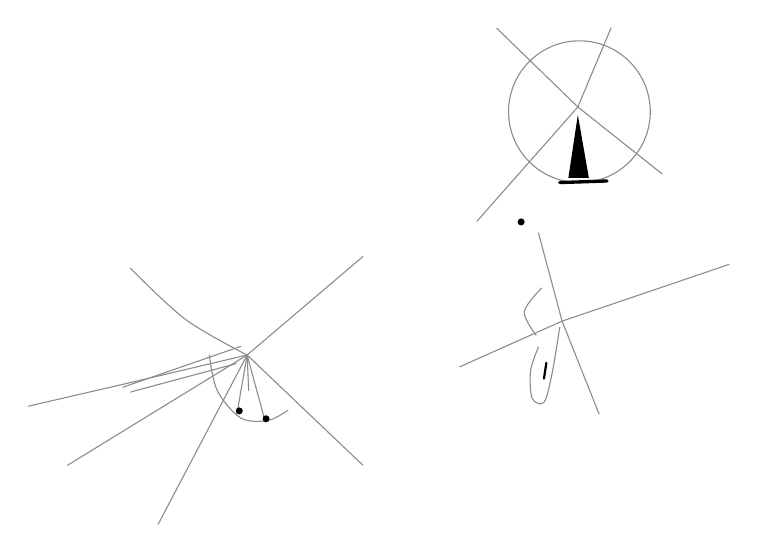
\begin{tikzpicture}[x=1mm,y=1mm,line cap=round,line join=round,font=\small]
\draw[pencil] plot[smooth, tension=0.55] coordinates {(13,-30.5) (20,-37) (27.8,-41.5)};
\draw[pencil] (27.8,-41.5) -- (42.5,-29);
\draw[pencil] (0,-48) -- (13,-45) -- (27.8,-41.5);
\draw[pencil] (12,-45.6) -- (27,-40.4);
\draw[pencil] (13,-46.2) -- (26.4,-42.6);
\draw[pencil] (27.8,-41.5) -- (5,-55.5);
\draw[pencil] (27.8,-41.5) -- (16.5,-63);
\draw[pencil] (27.8,-41.5) -- (42.5,-55.5);
\draw[pencil] plot[smooth, tension=0.55] coordinates {(23,-41.5) (24,-46) (27,-49.5) (30.5,-49.8) (33,-48.5)};
\draw[pencil] (27.8,-41.5) -- (26.5,-49);
\draw[pencil] (27.8,-41.5) -- (30,-49.6);
\draw[pencil] (27.8,-41.5) -- (28,-46);
\node[pt] at (26.8,-48.6) {};
\node[pt] at (30.2,-49.6) {};
\draw[pencil] (70,-10.6) circle[radius=9];
\draw[pencil] (59.5,0) -- (69.8,-10) -- (80.5,-18.5);
\draw[pencil] (74,0) -- (69.8,-10) -- (57,-24.5);
\fill (69.8,-11) -- (68.6,-19) -- (71.2,-19) -- cycle;
\draw[very thick] (67.5,-19.6) -- (73.5,-19.4);
\node[pt] at (62.6,-24.6) {};
\draw[pencil] (54.8,-43) -- (67.8,-37.2) -- (89,-30);
\draw[pencil] (64.8,-26) -- (67.8,-37.2) -- (72.5,-49);
\draw[pencil] plot[smooth, tension=0.55] coordinates {(65.2,-33) (63,-36) (64.5,-39)};
\draw[pencil] plot[smooth, tension=0.55] coordinates {(67.5,-38) (66.5,-44) (65.5,-47.5) (64,-47) (63.8,-43.5) (64.8,-40.5)};
\draw[thick] (65.8,-42.5) -- (65.5,-44.5);
\end{tikzpicture}
\end{document}
